
When the string is plucked, it will create travelling waves on the string that reflect at both ends, creating standing waves. The frequency of the standing waves with the longest wavelength is the fundamental frequency, also called the first harmonic. This is the lowest frequency, and there will usually be other higher harmonics that when combined create the characteristic timbre of the electric guitar. 
\begin{figure}[h]
    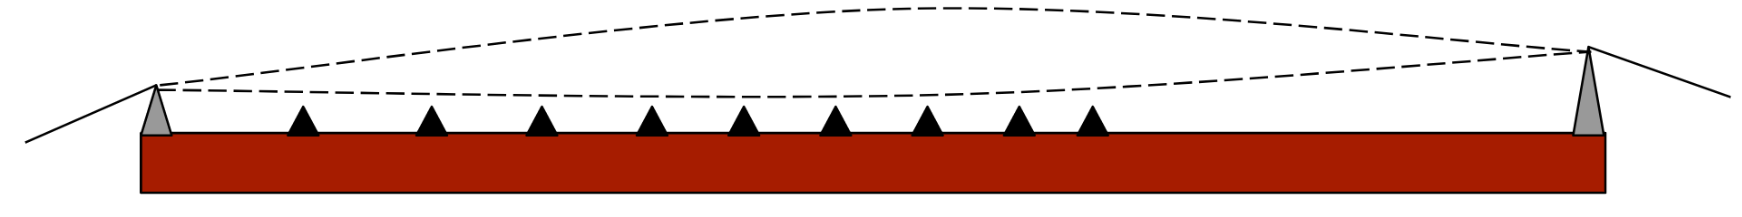
\includegraphics[width=\textwidth]{./ee/fig2.png}
    \caption{The “open” string (not fretted) is plucked and vibrating at its fundamental frequency.}\label{fig2}
\end{figure} 

The fundamental frequency $f_0$ of a string is determined by this formula
\begin{equation}\label{eqn1}
    f_0 = \frac{v}{\lambda}
\end{equation}
where $v$ is the speed of the wave on the string and $\lambda$ is the wavelength. \cite{eqn1} \par 
From Figure \ref{fig2} we see the wavelength is double the length of the guitar - the “scale length” $l$ . Therefore \begin{equation}\label{eqn2}
    \lambda = 2l
\end{equation}
The speed of the wave $v$ on a stretched string with tension $T$ can be determined by the equation:
\begin{equation}\label{eqn3}
    v = \sqrt{\frac{T}{\mu}} 
\end{equation}
Where $\mu$ is the linear density of the string (mass of string per unit length) \cite{eqn3}\par
Substitute (\ref{eqn2}) and (\ref{eqn3}) into (\ref{eqn1}) we get the expression for the frequency of an open string
\begin{equation}\label{eqn4}
    f_0 = \frac{1}{2l}\sqrt{\frac{T}{\mu}}
\end{equation}
